%%%%%%%%%%%%%%%%%%%%%%% file template.tex %%%%%%%%%%%%%%%%%%%%%%%%%
%
% This is a template file that is originally from a physics journal (The European Physical Journal Special Topics)
%
% Copy it to a new file with a new name and use it as the basis for your report
%
%
%
\documentclass[epjST]{svjour}
%
\usepackage{graphicx}
\usepackage{amsmath}
\usepackage{amsthm}
\usepackage{amssymb}
\usepackage{amsfonts}
\usepackage{subcaption}
\usepackage{algorithm}
\usepackage{algpseudocode}
\usepackage{array}
\usepackage{float}
\usepackage{hyperref}

%
\def\projectnb{}
\def\projectref{Cornea Stretch Energy}
\begin{document}
%
\title{Extracting the Human Cornea's Deformation Energy from Tonometer Captures of an Air Puff Exam}

\subtitle{Ecole Polytechnique - \projectref}
\author{Author: Ryan SFEILA\thanks{\email{ryan.sfeila@polytechnique.edu}}\\ Supervisor: Jean-Marc ALLAIN\thanks{\email{jean-marc.allain@polytechnique.edu}}}
\date{}
%
%\institute{Insert the first address here \and the second here \and ...}
%
\abstract{
% \emph{Write the Abstract as the final step of your work.}\\
% Identify the major objectives and conclusions, keywords, method used and major results in your project and assemble the information into a single paragraph containing no more than two or three short sentences.\\
% \emph{Hints}:\\
% - Omit background information, literature review, and detailed description of
% methods.\\
% - Remove extra words and phrases.\\
% - Revise the paragraph so that the abstract conveys only the essential
% information.
This project comes after the statistical analysis done by Wu Yifan under Professor Jean-Marc Allain's supervision on tonometer captures from ophthalmologists containing movies of human patient corneas subjected to air puffs for an exam typically done to recover the intra-ocular pressure. The dataset contains healthy corneas and corneas diagnosed with keratoconus disease. The goal of this project is to build upon the image processing and superficial statistical measures of thickness and characteristic lengths extracted from the videos to try and extract an energy evolution of the corneas using discretization and exclusively the tonometer captures with no further information on experimental control parameters.\\\\ \emph{Note that this document is still subject to change in light of new developments.}
\\\\
\textbf{Key words:} Discretization, Cornea Segmentation, Energy Proxy, Image Processing, Cornea Fit Validation, Cornea Waveforms.}
 %end of abstract
%
\maketitle
\tableofcontents
\section{Introduction and Contextualization}
Keratoconus disease is a disorder that affects the cornea and manifests itself with a thinning of the cornea and a gradual outward bulging of its shape until it reaches a cone-like shape. It is typically diagnosed by ophthalmologists through corneal topography - which puts in evidence the eccentric curvature of affected corneas - and keratoscopy - which puts in evidence the thinning of the cornea, typically in central regions. This shift in the mechanical properties cornea motivates an investigation into its energetic response to the applied air puff during the IOP exam, typically done thanks to a calibrated calculation of the tonometer's kinematic measurements. Full information on the air puff creation and exam parameters such as distances, patient head placement, and more would, in theory, be enough to solve the evolution using the principle of minimum potential energy. However, this would require accurate information on the cornea's local mechanical properties and the air puff's form throughout its interaction with the cornea, which motivates short-cutting this procedure to try and extract all the desired information from the movie, based on the principle that the shape evolution of the cornea should encode its energy's evolution up to a representation of energy. Throughout this project, we try to discretize our cornea into regions that we subsequently treat as independent segments or planes that have easily calculated energies, and the extremities of which simultaneously affect several neighboring finite elements - the aggregation of these effects results in a global energy evolution. We do this by building a simple proxy of energy, depending only on the shape of the discrete mesh into which our cornea is decomposed, and separating bending and stretching effects. The idea is that the proxy of relative energy is enough to detect trends that could help us distinguish between healthy and keratoconus-affected corneas.
\\\\
Throughout this report, we introduce the reader to all approaches tried and weaknesses/gains discovered in chronological order.
\section{The One-Dimensional Cornea Approach}
Seeing as we are already building a proxy of energy, we can start by treating our cornea as a one-dimensional object, moving in a two-dimensional plane as observed in the cross-section captured by the tonometer (which is actually a reconstruction.) Subsequently, we could assume a certain symmetry - such as axial symmetry in the simplest case - and build a two-dimensional surface cornea in a three-dimensional space, but this may not add to the trend we recover from the one-dimensional illustration as it already contains stretching and bending, the main contributors to the mechanical energy of the cornea.
\section{Previous Work}
This project begins after the groundwork for the raw video processing has already been done by Wu Yifan, who interned under Jean-Marc Allain's supervision. Though the primary goal of that project was to extract characteristic movie lengths and measurements, it required the development of image processing tools that we use to numerically treat our corneas in this project.
\subsection{Frame Extraction and Color Thresholding}
The first element of raw data processing implemented is the extraction of frames from the videos and the thresholding of the images so that we can obtain white corneas and black surroundings, making it easier to find the cornea when iterating over the image as an array of pixels. This process is illustrated in \autoref{fig:old40} and \autoref{fig:40}.
\begin{figure}[h]
    \centering
    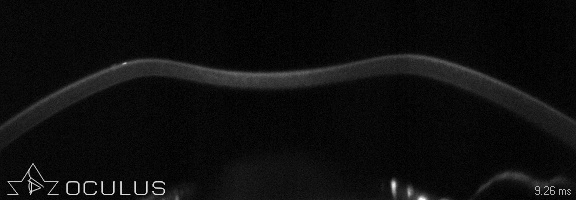
\includegraphics[width=0.6\linewidth]{figures/processing/image40old.jpg}
    \caption{Frame From Tonometer Movie Before Processing}
    \label{fig:old40}
\end{figure}
\begin{figure}[h]
    \centering
    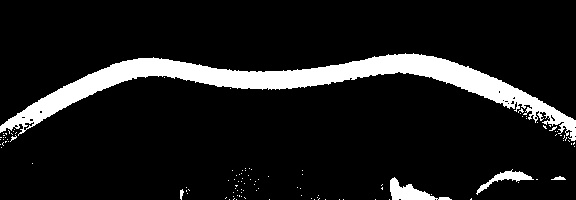
\includegraphics[width=0.6\linewidth]{figures/processing/image40.jpg}
    \caption{Frame From Tonometer Movie After Thresholding}
    \label{fig:40}
\end{figure}
\subsection{Waveform Extraction}
Another important tool to go from a cornea illustration to a numerically manipulable line on our grid is the extraction of the cornea's ``waveform'', as one would naturally refer to it in this one-dimensional approach. We do this by going over each vertical line of the frames and going from top to bottom, looking for the first and last white pixels - with a robustness mechanism requiring them to respectively be followed and preceded by 100 white pixels to avoid catching noise - before recording these as part of the upper and lower waveforms and building the middle, ``representative'' waveform by averaging the positions of the upper and lower waveform arrays. An illustration is shown in \autoref{fig:wavs}.
\begin{figure}[h]
    \centering
    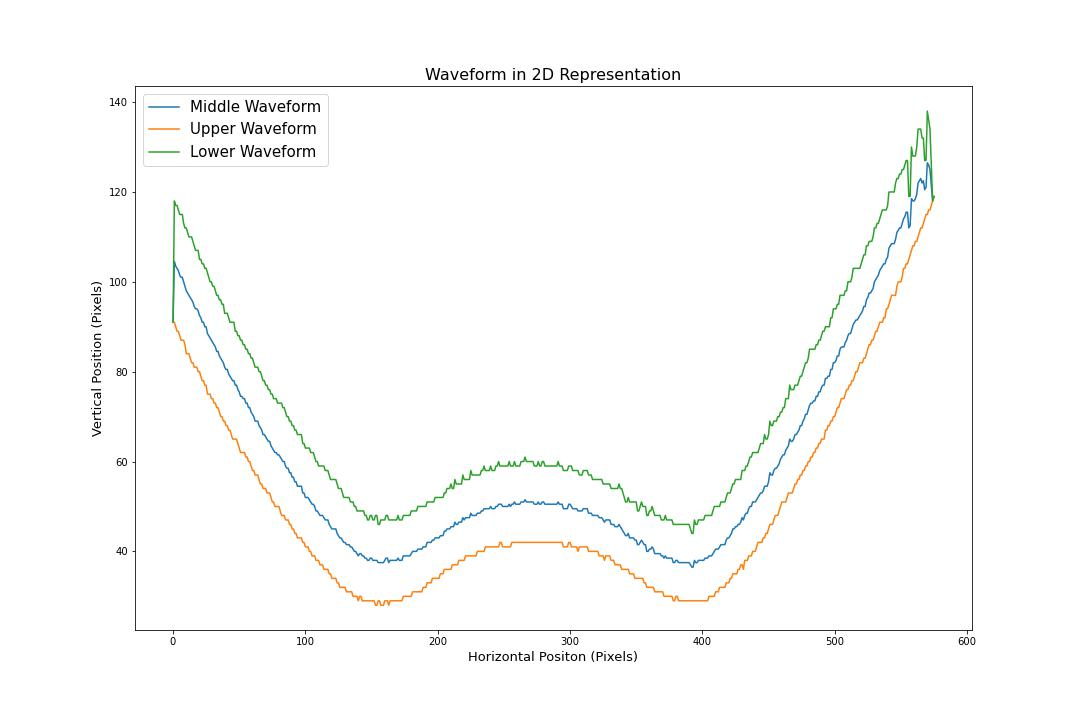
\includegraphics[width=1\linewidth]{figures/processing/IGNORE_1.jpg}
    \caption{Waveform Extraction From Frames. Axes Appear Inverted Due to the Way a Picture is Read as an Array by the Pre-Processing Library.}
    \label{fig:wavs}
\end{figure}
\section{Procedure Outline}
This section is dedicated to outlining the undertaken procedure and highlight the expected challenges and how we will tackle them. Consider the two-dimensional grid on which we deal with our numerical cornea. We choose a set of $x -$ positions (along the horizontal axis) and track the vertical movement of the cornea at these x-positions. On the first frame of a movie, we place what we will refer to as ``nodes'' on the cornea. Say we place a number $N$ of nodes excluding our left and right extremities, so that the total of $N+2$ nodes including the extremities of the cornea form $N+1$ segments, the energies of which we will treat as simple one-dimensional elastic objects.
\subsection{A First Consideration: The Elastic Stretch Energy}
Consider for instance the elastic stretching energy of the segment elements - we will treat the bending energy in a later phase on its own, to find separate trends in these two energetic aspects. We will try to track the movement of these nodes over frame evolution to track the segments' length and consequently energy evolutions.
\subsection{Frame 0: The Calibration Frame}
We first take the first frame of a given video. We choose our $x-$ positions and find the cornea $y$ position at these horizontal points, and we decide that these are our nodes. We can consequently get the rest length of our segments. These are indeed ``pseudo-rest'' rest lengths because they result from the pressure balance of the IOP and external pressure, but these do not change throughout the experiment. We also give every segment a stretching stiffness that is equal to the rest length reciprocal, an analog to mechanics problems with springs of identical characteristics with varying lengths connected in series and which each have a stiffness that is inversely proportional to their length - if you chop off half a spring, you are left with half a spring with double the stiffness in $\rm N/m$. Now, we know where the nodes, and more importantly their rest lengths and stiffnesses, which are experiment constants.
\subsection{The Evolution}
On all subsequent frames, the vertical positions tracked at our chosen $x-$ positions during calibration do not yield the node positions, because the nodes move horizontally as well as vertically. These horizontal displacements are our problem's $N$ unknowns (we assume the extremities do not move horizontally, just vertically, and we re-adjust this vertical global shift due to the cornea's global movement.) The resultant vertical shift due to horizontal displacement is fully parametrized by this horizontal displacement since once we know the node's final $x-$ location, we see where the cornea is at this position and we have the node's $(x,y)$ coordinates, from which we can get the new segment lengths and then their compression/elongation energies from Hooke's law. This reconstruction of the nodes after their movement is the main challenge of this project, and the later sections illustrate the attempts made for this reconstruction. But what dictates cornea node movements?
\subsubsection{The Principle of Minimum Potential Energy}
Given a deformation fully described by a new waveform on a later frame of a video, the cornea points have moved such that the aggregate energy of the system is minimized; this is the manifestation of the celebrated principle of minimal potential energy, which is central to this project's feasibility. Hence we have reduced our problem on a late frame to a $N-$ dimensional optimization problem which is easily solved by smart initial guesses and classic iterative algorithms implemented by numerous Python libraries such as the \texttt{scipy.optimize} module.
\subsubsection{A Well-Conditioned Problem}
Our total potential energy writes as the sum of segment energies, which is an expression containing all node locations and displacements. All partial derivatives of the energy must be zero at the optimum, giving us $N$ nonlinear equations to solve with $N-$ unknowns so that our problem is well-conditioned. The exact expression of the potential energy depends on our chosen reconstruction, and this is outlined in later sections. Had we not parametrized the vertical movement by the horizontal one, we would have underspecified our system, and our algorithm would be able to stay at zero energy. 
\subsubsection{The Smart Guess for Iterative Optimization}
\label{sec:smart}
On the first frame, a natural guess to stat iteration is no displacement, since on this frame 0 displacement brings zero new lengths, which brings zero additional energies - note that from the mere form of elastic potential energy, all energies on all frames are bounded from below by zero, as we are using a proxy of relative energy calibrated on the first frame. On the subsequent frames, we use the displacements that result from the optimization on the previous frame, a natural guess for a finely decomposed video.
\section{Getting the Cornea Waveform Function}
From the way the pre-processing is done, what we refer to as the extracted waveform is an array of $y-$ positions, the size of the image in pixels. Hence, we can only access the cornea vertical locations at $x=0,..,575$. In order to get the cornea vertical positions at any horizontal position and on a given frame, we fit the waveform array with a polynomial of the fourth degree - this is the degree that seemed to do the best job empirically regarding truly representing the shape and not developing more than two peaks throughout the experiment as polynomials of higher order started doing beyond a certain frame, leading to undesired localizations of displacement and energy on the borders. We first did this for the middle waveforms, before realizing that the upper waveforms were much smoother because the noise from the lower waveform ruined our middle one. We use the \texttt{np.polyfit} least-squares polynomial regression and get our wavefunctions given by functions defined on $[0,575]$. An example is illustrated in \autoref{fig:polyfit}.
\begin{figure}[h]
    \centering
    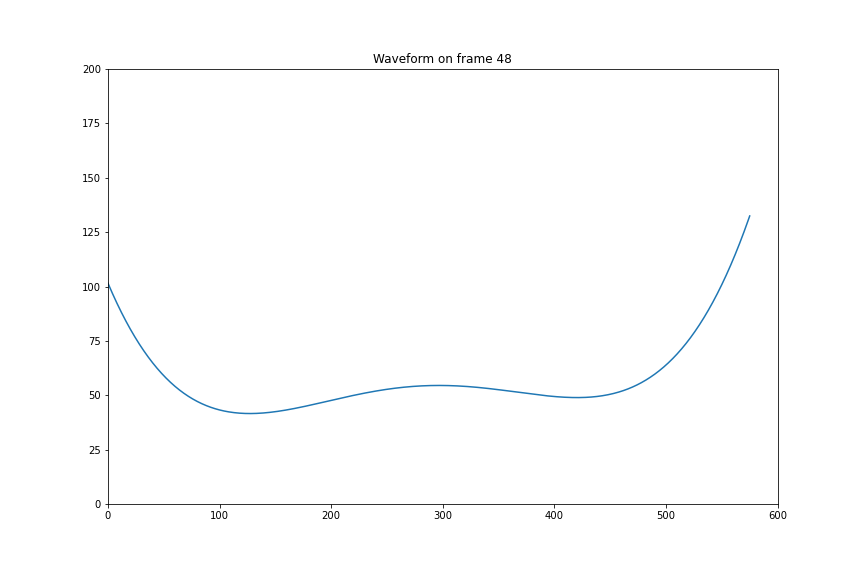
\includegraphics[width=0.9\linewidth]{figures/processing/48.png}
    \caption{Waveform Given by Polynomial Fit of Upper Waveform Array.}
    \label{fig:polyfit}
\end{figure}
Once we have these polynomials, our first, straightforward approach consists of the following.
\begin{enumerate}
    \item Place $N$ points along the $x-$ axis. We chose $N= 100$ to start with and use \texttt{np.linspace} to have equidistant points on the horizontal line.
    \\\item Use the global polynomial fit to retrieve the corresponding array of $y-$ positions.
    \\\item Send these arrays, the prerecorded rest lengths, and the prerecorded stiffnesses to the minimization algorithm to get the equilibrium displacements.
\end{enumerate}
Before tackling fit quality issues, we must answer the question on the parametrization of vertical displacement by the horizontal displacements, which we denote $(u_i)_{i = 1,...,N}$. We also denote $u_0:=0$ and $u_{N+1}:= 0$ the null displacement of the edges for representation purposes (we have $N+2$ nodes counting the extremities that do not serve as unknowns but as known system parameters.) The way the optimization is performed is by writing an explicit form of the potential energy that is a function $U:\mathbb{R}^N\to \mathbb{R}$ that maps displacements to resultant energy, before passing this objective function to \texttt{scipy.optimize.minimize} for optimization using classic iterative algorithms (BFGS is the default optimization algorithm.) What we chose to do to determine how much a node is believed to have moved along $y$ provided it has moved along $x$ by $u_i$ is illustrated in the following procedure for calculating potential energy of a given waveform, which comes from given frame - we do this procedure on all frames of a movie.
\begin{itemize}
    \item We are given, from frame 0, the chosen $x-$ positions to track including the cornea edges, and we denote them $(x_i)_{i=0,...,N+1}$. We denote $(S_i)_{i=1,...,N+1}$ the $N+1$ segments formed by the initial node placement at the $x-$ positions. Using the cornea waveform, we compute each node's starting vertical location and get the segment reference lengths $(l_i)_{i=1,...,N+1}$. We use these lengths and get the corresponding relative stiffnesses $(k_i)_{i=1,...,N+1}$.All these are recorded.
    \\\item Over a later frame, we use the fitted waveform to get the cornea vertical locations $(y_i)_{i=0,...,N+1}$ at the $(x_i)_i$ positions, and propose horizontal displacements $(u_i)_{i=1,...,N}$ of the free nodes as outlined as outlined in \autoref{sec:smart} over which we will iterate. We use to pass these displacements - the problem variables - to our draft of a potential energy function. We denote $u_0 = u_{N+1} = 0$ the forced zero displacements of the cornea edges.
    \\\item We iterate over the segments to compute their energy. On segment $i$, the nodes forming the left and right extremities have the new $x-$ positions $x_{i-1} + $ and $x_i$ respectively. The algorithm uses a basic linear extrapolation of the node's actual vertical position; the slope of $S_i$ multiplied by $u_{i-1}$ is the change from $y_{i-1}$ of the vertical position of the left segment extremity and the slope of $S_i$ multiplied by $u_{i}$ is the change from $y_{i}$ of the vertical position of the right segment extremity.
    \\\item We use these new positions to compute the new segment length and find the stretch energy using the stiffness and rest length before aggregating the segment energies.
\end{itemize}
We make the following observations on this approach.
\begin{itemize}
    \item This approximation assumes a very large scale of variation of the cornea's tangent, which is not a very bad assumption with a fine enough discretization.
    \\\item As we move from one segment to the next, a node's extrapolated position is computed twice, using two different slopes. We assume these slopes won't be too different on a fine enough discretization, and that this double computation could serve as an ``averaging'' effect to remove preceding segment bias.
    \\\item In this framework, the potential energy function that is minimized writes:
    \[
    U = \sum_{i=1}^{N+1} \frac{1}{2}k_i \: \left(\sqrt{(x_i-x_{i-1} + u_i-u_{i-1})^2+\left(y_i+u_i \frac{y_i-y_{i-1}}{x_i-x_{i-1}}-y_{i-1}-u_{i-1} \frac{y_i-y_{i-1}}{x_i-x_{i-1}}\right)^2}-l_{i}\right)^2
    \]
    \item We sanity check our optimizer's convergence to the desired minimum by comparing the results with a solver of a system of non-linear equations that solves the system given by:
    \[
    \frac{\partial U_s}{\partial u_i} = K_i \: \left(\sqrt{(x_i-x_{i-1} + u_i-u_{i-1})^2+\left(y_i+u_i \frac{y_i-y_{i-1}}{x_i-x_{i-1}}-y_{i-1}-u_{i-1} \frac{y_i-y_{i-1}}{x_i-x_{i-1}}\right)^2}-l_{0,i}\right)
    \]
    \[
    \times
\frac{(x_i-x_{i-1}+u_i-u_{i-1})+\left(y_i+u_i \frac{y_i-y_{i-1}}{x_i-x_{i-1}}-y_{i-1}-u_{i-1} \frac{y_i-y_{i-1}}{x_i-x_{i-1}}\right)\cdot \frac{y_i-y_{i-1}}{x_i-x_{i-1}} }{\sqrt{(x_i-x_{i-1} + u_i-u_{i-1})^2+\left(y_i+u_i \frac{y_i-y_{i-1}}{x_i-x_{i-1}}-y_{i-1}-u_{i-1} \frac{y_i-y_{i-1}}{x_i-x_{i-1}}\right)^2}}
    \]
    \[
    -K_{i+1} \: \left(\sqrt{(x_{i+1}-x_{i} + u_{i+1}-u_{i})^2+\left(y_{i+1}+u_{i+1} \frac{y_{i+1}-y_{i}}{x_{i+1}-x_{i}}-y_{i}-u_{i} \frac{y_{i+1}-y_{i}}{x_{i+1}-x_{i}}\right)^2}-l_{0,i+1}\right)
    \]
    \[
    \times
\frac{(x_{i+1}-x_{i}+u_{i+1}-u_{i})+\left(y_{i+1}+u_{i+1} \frac{y_{i+1}-y_{i}}{x_{i+1}-x_{i}}-y_{i}-u_{i} \frac{y_{i+1}-y_{i}}{x_{i+1}-x_{i}}\right)\cdot \frac{y_{i+1}-y_{i}}{x_{i+1}-x_{i}} }{\sqrt{(x_{i+1}-x_{i} + u_{i+1}-u_{i})^2+\left(y_{i+1}+u_{i+1} \frac{y_{i+1}-y_{i}}{x_{i+1}-x_{i}}-y_{i}-u_{i} \frac{y_{i+1}-y_{i}}{x_{i+1}-x_{i}}\right)^2}}
    \]
    We get similar results and conclude that the potential energy is written properly under this framework's assumptions. The two terms above appear because of each node's effect on the energy of two segments, an effect central to the convergence of the algorithm.
\end{itemize}
\section{Failure of The Global Fit and Linear Extrapolation Scheme}
After attempting to recover the global energy's evolution over the video's evolution in frames, we obtain noisy plots, an example of which is illustrated in \autoref{fig:noise1}
\begin{figure}[h]
    \centering
    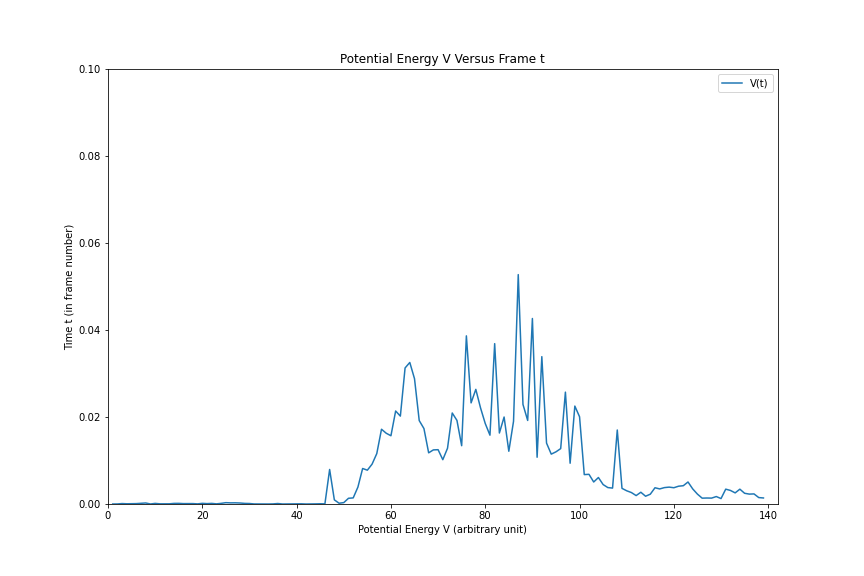
\includegraphics[width=0.8\linewidth]{figures/minimization1/TimeEvolution_up.png}
    \caption{Evolution of Potential Energy Under First Proposed Scheme}
    \label{fig:noise1}
\end{figure}
Unfortunately, the noise is far too intense to detect any characteristic trend. This motivates a series of diagnostic tests before proposing a new approach in which we attempt to treat the sources of error in our simulation. Some of the potential culprits could include the following.
\begin{itemize}
    \item A bad, non-representative global fit of the waveform on most frames.
    \\\item Our potential energy function is ill-conditioned.
    \\\item The boundary conditions of fixed edges do not hold true on the tonometer captures owing to incomplete cornea representation in the available data.
\end{itemize}
\subsection{Testing the Potential Energy Function on a Stretching Spring}
We can first attempt to detect obvious performance issues in our potential energy function by hardcoding an example of a line stretching and contracting. This, of course, doesn't justify the perfect, proper convergence of the algorithm, but can motivate troubleshooting elsewhere. We get a smooth evolution as expected in \autoref{fig:line1}.
\begin{figure}[h]
    \centering
    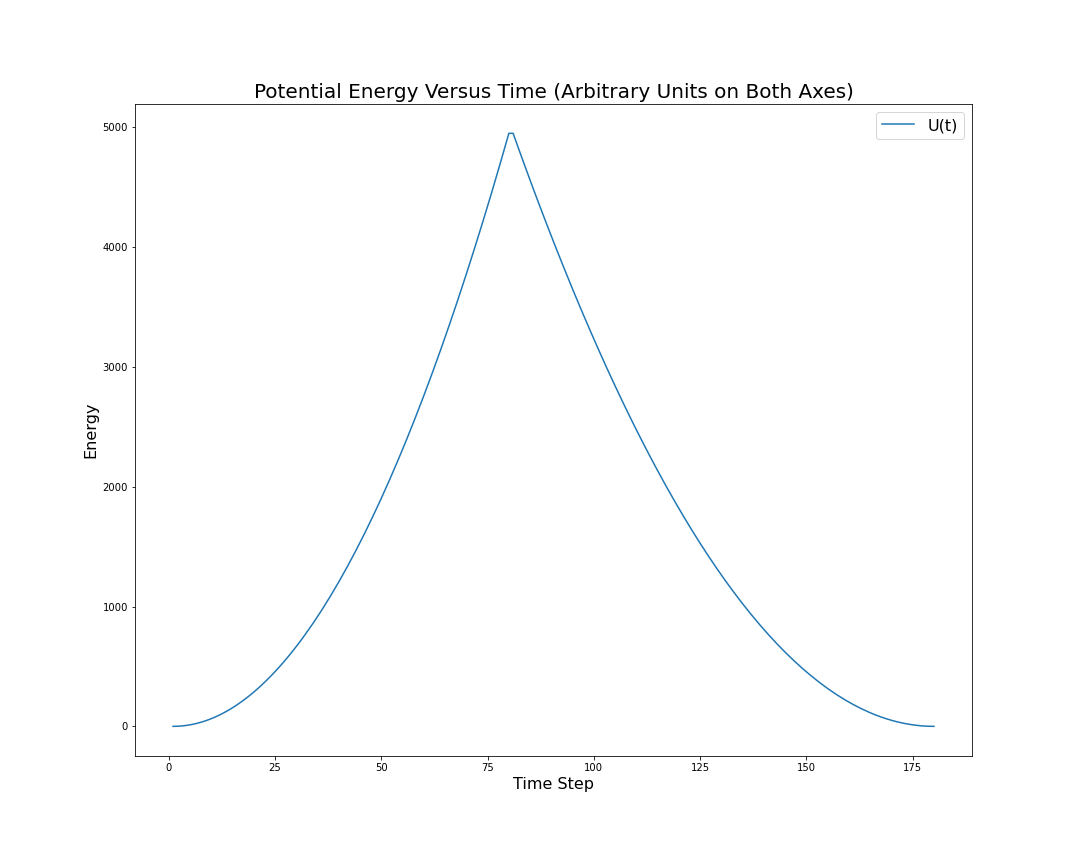
\includegraphics[width=0.8\linewidth]{figures/minimization1/noise_energy_time_plot.png}
    \caption{Hardcoded Stretching Line Case's Resultant Energy Evolution}
    \label{fig:line1}
\end{figure}
The same results from hardcoding simple examples such as parabolas and semi-circles in simple cases. We even maintain the curve's smoothness after introducing noise on the $x$ and $y$ arrays of about 5\% the total available length on each frame passed to the minimization algorithm.
\subsection{Reconstruction Error}
We can try to spot, with the naked eye, a non-smooth evolution of the global fits by creating a movie of the waveforms. We obtain movies with some evident twitching at the borders, hinting undesired local error phenomena near the borders. We then plot the absolute difference between the directly obtained $y-$ positions of the cornea at each pixel and the fitted curve's corresponding $y-$ predictions and recover non-negligible error, which begins to reveal to low-quality results. This per pixel deviation plot is done on each frame to create a movie of the error versus $x-$ location graph, and toward the middle of the air puff experiment, we get error plots similar to that illustrated in \autoref{fig:error1}.
\begin{figure}
    \centering
    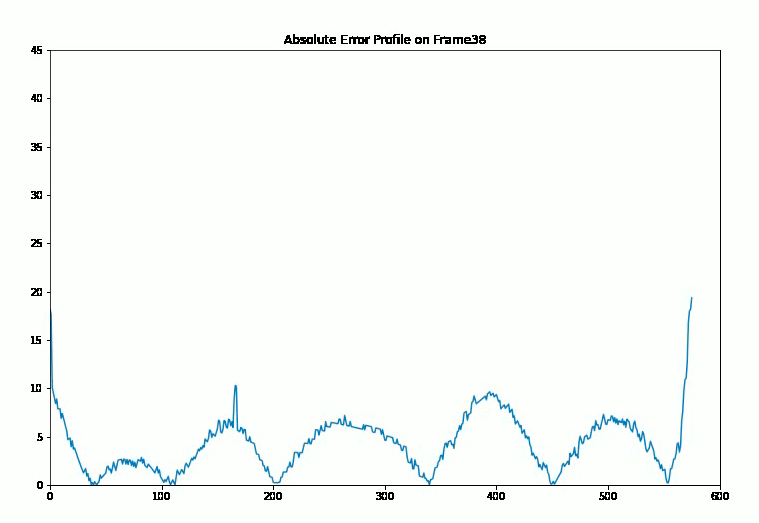
\includegraphics[width=0.8\linewidth]{figures/minimization1/Screen Shot 2024-07-29 at 10.38.13 PM.png}
    \caption{Absolute Difference Between Measured and Fitted Horizontal Cornea Positions On All Pixels at One of the Frames Used to Make an Evolution Movie of this Error Profile Using \texttt{cv2}.}
    \label{fig:error1}
\end{figure}
We can check the implications of these inhibiting edge effects by plotting the individual segment energies' evolution with time, which we also represent on a movie of the graph of Potential Energy Versus Segment Number as the frames evolve. An interesting phenomenon of energy localization on the border is illustrated in \autoref{localization1}. We do not know what exactly to expect from this evolution, which may go against our intuition in the absence of bending energy, but the fact that the energy is localized on the edges during the entire clip hints at errors in that area. Furthermore, the movie of these plots doesn't evolve very smoothly.
\begin{figure}
    \centering
    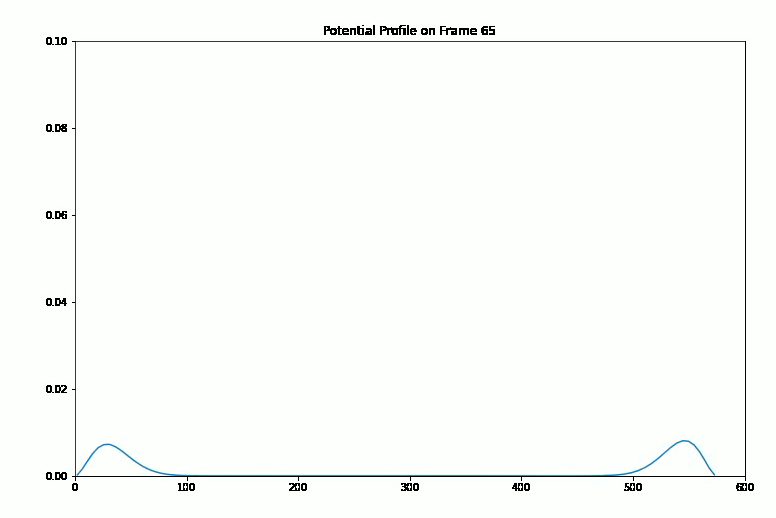
\includegraphics[width=0.8\linewidth]{figures/minimization1/Screen Shot 2024-07-29 at 10.44.40 PM.png}
    \caption{Potential Energy Versus $x-$ Position (Sampled at the Segment Midpoint Locations). The vertical axis is the energy and the horizontal one is the location of the segment midpoint.}
    \label{fig:enter-label}
\end{figure}
\subsection{Issues to Investigate Following the Initial Attempt}
Our subsequent efforts will be focused in treating the following.
\begin{enumerate}
    \item We will try to track cornea vertical locations more accurately, such as avoiding global fitting before minimization so that an accurate array of $(y_i)_i$ for a given frame is passed to the minimizing algorithm. Upon recomputing the resultant vertical locations of the nodes, which may not be at integer values of $x$ - for which we have no waveform array components - we may have to use a local fitting or polygon approximation of the curve using the known points that are the waveform arrays before fitting.
    \\\item We will try to develop schemes to account for the possible movement of the edges out of frame, a phenomenon suggested to exist by the twitching waveforms and instability at the edges. We had assumed the whole eye almost entirely stays within the frame, but this may not be the case as it turns out.
\end{enumerate}
\subsection{Summary of First Algorithm}
\label{algos1}
In this section, we outline what has been done so far in pseudo-code to have an easier visualization of the subsequent of our approach.
\begin{algorithm}
    \caption{The Potential Energy Function - A Linear Extrapolation of the Nodes}
    \label{alg:pot1}
    \begin{algorithmic}[1]
        \Require Tracked Horizontal Positions $x_i$ (Including Edges)
        \Require Cornea Vertical Positions at Tracked Horizontal Locations $y_i$
        \Require Segment Rest Lengths $l_i$
        \Require Stiffnesses $k_i$
        \State Initialize Energy Array $(E_i)_{i=1,...,N+1}; E_i = 0\:\forall i$
        \For{$i=0,...,N$}
        \State $\text{Slope}\gets \text{segment\_slope}([x_i,y_i],[x_{i+1},y_{i+1}])$
        \State $\text{Segment Left}\gets (x_{i}+u_{i}\:,\: y_i + u_i \times \text{Slope})$
        \State $\text{Segment Right}\gets (x_{i+1}+u_{i+1}\:,\: y_{i+1} + u_{i+1} \times \text{Slope})$
        \State $\text{New Length}\gets \text{euclidean\_distance}(\text{Segement Left , Segment Right})$
        \State $E_i\gets 0.5\times k_{i+1} \times (\text{New Length} - l_{i+1})^2$\Comment{ Indexing Conventions in Require}
        \EndFor\\
        \Return sum($E_i$)
    \end{algorithmic}
\end{algorithm}
\begin{algorithm}
    \caption{Get The Potential Energy on a Given Frame}
    \label{alg:frampot1}
    \begin{algorithmic}[1]
        \Require Tracked Horizontal Positions $x_i$ (Including Edges)
        \Require (Path to) Frame
        \Require Segment Rest Lengths $l_i$
        \Require Stiffnesses $k_i$
        \Require Minimizer scipy.optimize.minimize; abbreviate as Minimize
        \Require Initial Guess for Displacement of FREE NODES $(u_i)_{i=1,...,N}$
        \State $(y_{0,i})_{i=0,...,N+1} \gets \text{get\_waveform\_array(Frame)}$
        \State $(y_i)_{i=0,...,N+1} \gets \text{global\_polynomial\_fit}(y_{0,i})$
        \State $\text{Fixed Arguments}\gets (l_i, k_i, u_0=0, u_{N+1}=0)$
        \State $\text{Displacements} \gets \text{Minimize}(\text{Over : }(u_i)_{i=1,...,N},\text{Function : \autoref{alg:pot1} }, \text{ With Fixed parameters : Fixed Arguments})$
        \State $\text{Frame Energy}\gets \text{\autoref{alg:pot1}} \text{ Evaluated at Resultant Displacements}$
        \\\Return Displacements, Frame Energy
        
    \end{algorithmic}
\end{algorithm}
\begin{algorithm}
\label{alg:potev1}
    \caption{Get The Potential Energy Evolution}
    \begin{algorithmic}[1]
        \Require Video Name, Path to Processed Frames, Total Number of Images
        \Require Array of $N$ Horizontal Locations to Place Nodes Including Extremities $(x_i)_{i=1...,N}$
        \State Get Frame 0 Calibration; \begin{itemize}
            \item $y_{0,i} \gets \text{get\_waveform}(\text{Frame 0})$
            \item $y_i\gets \text{polynomial\_fit}(y_{0,i})$
            \item $l_i\gets \text{euclidean\_distances}(x_i,y_i)$
            \item $k_i = 1\: \forall i$
            \item $k_i \gets k_i/l_i$
        \end{itemize}
        \State Guess := Array of 0s
        \State Energy Time Series Array := Array of 0s
        \State Array of Displacements := Array of Zeros Size: (Total Images, $N$)
        \For{$t = 1$,...,Total Images}
        \State $D,\:U\gets \text{ \autoref{alg:frampot1} }(x_i, \text{Frame $t$}, l_i, k_i, \text{ Guess })$
        \State $\text{Guess} \gets D$
        \State $\text{Dispalcements}[t]\gets D$
        \State $\text{Energy}[t]\gets U$
        \EndFor
        \\
        \Return Displacements, Energy
    \end{algorithmic}
\end{algorithm}
\section{Avoiding the Global Fit}
A first attempt to reduce experiment noise is to refrain from performing the global fit which redefines our cornea's vertical locations in a sub-optimal manner as highlighted in the above diagnostic tests, especially \autoref{fig:error1}. 
\subsection{Using the Waveform Array}
The waveform-fetching function originally contained the global fitting scheme. This was necessary since our chosen horizontal points to track softened landed between pixels, where the discrete vertical locations array doesn't yield explicit information. One thing we can do is to force our $x-$ points to be placed on a whole number of pixels so that we can omit the fitting part and just index the array returned by the waveform fetcher using the $x-$ positions in pixels as indices since the initial array contains a $y-$ node for each pixel, but we do not work with all pixels due to computational limitations and in hopes that such measures aren't necessary. A simple way to do this is to choose the number of nodes and the interval, find the separation and round it down, then place the nodes and leave all the remainder for the final node separation between the last free node and 575. At this stage, we can already rerun the algorithm as outlined in \autoref{algos1} and omit the global fitting, still using the linear extrapolation. We obtain something a bit less noisy but not good enough for trend recovery, but the approach motivates staying away from polynomial fitting at least on a cornea-wide scale. An example of the results is shown in \autoref{fig:ev2} with little graph care as it was quickly discarded.
\begin{figure}[h]
    \centering
    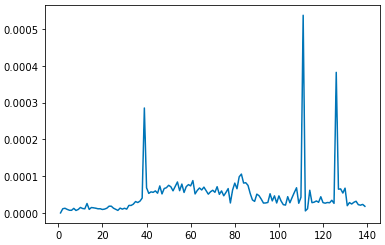
\includegraphics[width=0.5\linewidth]{figures/minimization2/app2.png}
    \caption{Potential Energy Evolution with No Global Fitting and a Linear Node Extrapolation\\
    Energy on the Vertical Axis and Frame on the Horizontal. Singularities ruin the variation illustration, but the noise apparent even on this scale is demotivating and suggests something different.}
    \label{fig:ev2}
\end{figure}

\subsection{Reconstructing Node Final Locations Using a Series of Local Fits}
Now that we pass the $(y_i)$ argument to the potential energy function without a global fit and in light of \autoref{fig:ev2}, we propose to reconstruct the final vertical position of each node by using a local polynomial fit of the nearby region rather than the entire cornea. We rewrite the potential energy that is minimized as follows.
\begin{algorithm}
    \caption{Potential Energy Function - Local Fitting Rather than Linear Local Linear Extrapolation}
    \label{locfit}
   \begin{algorithmic}[1]
        \Require Tracked Horizontal Positions $x_i$ (Including Edges)
        \Require Cornea Vertical Positions at Tracked Horizontal Locations $y_i$
        \Require Segment Rest Lengths $l_i$
        \Require Stiffnesses $k_i$
        \State Initialize Energy Array $(E_i)_{i=0,...,N+1}; E_i = 0\:\forall i$
        \For{$i=1,...,N$}
        \State $\rm index\_left := \max(i-5,0)$
        \State $\rm index\_right := \min(i+5, 575)$
        \State $P\gets \rm polynomial\_fit$ $(x[\text{min\_index : max\_index}], y[\text{min\_index : max\_index}])$
        \State $S_i$ :=( $x_i+u_i$ , $P(x_i+u_i)$)
        \EndFor
          \For{$i=0,...,N$}
        \State $\text{New Length}\gets \text{euclidean\_distance}(S_i,S_{i+1} )$
        \State $E_i\gets 0.5\times k_{i+1} \times (\text{New Length} - l_{i+1})^2$\Comment{Indexing Conventions in Require}
        \EndFor\\
        \Return sum($E_i$)
    \end{algorithmic}
\end{algorithm}
Unfortunately, this approach involves a failure to solve the trivial case of no movement as the fit is a least squares and not an interpolating polynomial, which would be too noisy and unrepresentative. We get a bad signal and abandon the approach quickly.
\subsection{Reconstructing Node Final Locations By Interpolation Between Nearest Known Neighbors}
This section is dedicated to the best-performing potential energy scheme so far, compatible with the waveform array method as it only modifies the potential energy function. We now look to modify the linear extrapolation for something more stable than the local fitting and more accurate than the linear extrapolation.\\\\
Assuming that our discrete set of tagged x,y positions on a given waveform is a good proxy of its shape - which in turn requires a fine discretization and smooth recovery of the cornea points robust to image noise - we can dictate the vertical position of the cornea at any $x- $ (even off our pixels) by a linear interpolation performed between the two nearest tagged (x,y) pairs. In other words, rather than defining our cornea by a polynomial function or even a discrete array with local fitting reconstruction of unknown points which may be ill-conditioned, we can represent our cornea with a continuous function that is piecewise affine, or of degree one on each interval $(x_i,x_{i+1})$. Our potential energy would be transformed into the following with the interpolation auxiliary function. Note that the segments are also no longer rectilinear, and for consistency when fetching the new length, we sum the length of all rectilinear segments forming the cornea that are between any two points of the cornea.
\begin{algorithm}
    \caption{Interpolation - Cornea Rectilinear Representation - Extrapolation Beyond Edges}
    \label{alg:interp}
    \begin{algorithmic}[1]
        \Require Tagged Horizontal Positions $x_i$
        \Require Cornea Vertical Positions at Horizontal Positions $y_i$
        \Require A Horizontal Position to Map to a Vertical Position $X$.
        \If{$X<x_0$ or $X>x_{N+1}$}
        \If{$X<x_0$}
        \State $Y\gets \gets y_0 + (X-x_0)\times \text{Slope}(x_0,y_0,x_{1}, y_{1})$
        \ElsIf{$X>x_{N+1}$}
        \State $Y\gets \gets y_N + (X-x_N)\times \text{Slope}(x_N,y_N,x_{N+1}, y_{N+1})$
        \EndIf
        \Else
        \State Iterate to find $i$ such that $x_{i}\leq X\leq x_{i+1}$
        \State $Y\gets y_i + (X-x_i)\times \text{Slope}(x_i,y_i,x_{i+1}, y_{i+1})$.
        \EndIf
        \State\Return $Y$
    \end{algorithmic}
\end{algorithm}
\begin{algorithm}
    \caption{Segment Length Computation by Moving Along Cornea Function}
    \label{alg:distcorn}
    \begin{algorithmic}[1]
        \Require Tagged Horizontal Positions $x_i$
        \Require Cornea Vertical Positions at Horizontal Positions $y_i$
        \Require Start Point $(X_1, Y_1)$
        \Require End Point $(X_2, Y_2)$
       \State Iterate to find $ i=\arg\!\min_{i\:|\:x_i\geq X_1} x_i$
       \If{$x_i\geq X_2$}
       \State Distance := $\text{euclidean\_distance}(X_1, Y_1,X_2, Y_2)$
       \Else\State
       $k:=i$
       Distance := 0
       Current Point := $(X_1, Y_1)$
       \While{$x_k\leq X_2$ or $k\neq N+1$}
        \State $\text{Distance} \gets \text{Distance} + \text{euclidean\_distance}(\text{Current Point}, x_k,y_k)$
        \State
        $\text{Current Point}\gets (x_k,y_k)$
        \State
       $k\gets k+1$
       \EndWhile
       \EndIf
       \If{$X_2>x_{N+1}$}
       \State $\text{Distance}\gets \text{Distance} + \text{euclidean\_distance}(x_{N+1},y_{N+1}, X_2, Y_2)$
       \EndIf
       \State \Return Distance
    \end{algorithmic}
\end{algorithm}
\begin{algorithm}
    \caption{Potential Energy Function - Local Fitting Rather than Linear Local Linear Extrapolation}
    \label{potinterp}
   \begin{algorithmic}[1]
        \Require Tracked Horizontal Positions $x_i$ (Including Edges)
        \Require Cornea Vertical Positions at Tracked Horizontal Locations $y_i$
        \Require Segment Rest Lengths $l_i$
        \Require Stiffnesses $k_i$
        \State Initialize Energy Array $(E_i)_{i=1,...,N+1}; E_i = 0\:\forall i$
        \For{$i=0,...,N$}
        \State Segment Left :=( $x_i+u_i$ , $\text{ \autoref{alg:interp} }(x_i+u_i)$)
        \State Segment Right :=( $x_{i+1}+u_{i+1}$ , $\text{ \autoref{alg:interp} }(x_{i+1}+u_{i+1})$)
        \State $\text{New Length}\gets \text{ \autoref{alg:distcorn} }(\text{Segement Left , Segment Right})$
        \State $E_i\gets 0.5\times k_{i+1} \times (\text{New Length} - l_{i+1})^2$\Comment{ Indexing Conventions}
        \EndFor\\
        \Return sum($E_i$)
    \end{algorithmic}
\end{algorithm}

\noindent
We run this algorithm with 83 nodes (initially placed on pixels that we try to separate as much as possible to spread the noise on the jagged line that \autoref{alg:distcorn} runs over.) An example of a movie's evolution is shown in \autoref{fig:jagged1}.
\begin{figure}[h]
    \centering
    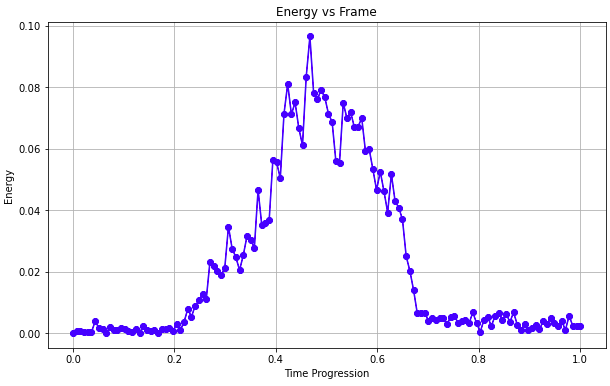
\includegraphics[width=0.8\linewidth]{figures/minimization2/jagged1.png}
    \caption{Evolution Resultant from the New Potential Energy Function Based on Interpolation}
    \label{fig:jagged1}
\end{figure}
We recover a much better curve than before, but still subject to some noise. This last bit of noise could be coming from two things.
\begin{enumerate}
    \item A noisy waveform (that we previously tried to smoothen with a representative fit unsuccessfully.)
    \\
    \item We haven't treated the issue of cornea extremities set at calibration leaving the frame under global contraction and expansion during the experiment. This is the focus of the next section.
\end{enumerate}
One thing we can do for the first point is to perform a grid search over the number of nodes to place. This requires higher computational power and will be done in the near future, at least for the maximal number of nodes 575. In the meantime, \autoref{vec} attempts to treat the global movement of the cornea along with its extremities, which we hoped don't move horizontally and move out of frame.
\section{Implementation of A Missing Portion Reconstruction}
\label{vec}
As mentioned above, a phenomenon to consider when designing the framework for our optimizer is the movement of our cornea edges in the horizontal direction. We make the following observations regarding cornea movement and local deformation which will motivate the design of an approach to encapsulate this information.
\begin{itemize}
    \item The cornea experiences a translational shift into the eye during the air puff exam, which on its own doesn't cause an issue with setting the horizontal shift of the edges to zero.
    \\\item This shift however isn't entirely translational but seems to involve of contraction of the cornea toward the center of the arc it forms on the plane. This could be a result of the air puff pushing the cornea back against tissue of muscle forcing the cornea to seemingly contract during the experiment before a rather evident outward expansion combined with a translational shift back to its original position.
    \\\item The shape of the cornea outside of central regions doesn't deform and can be recorded as fixed throughout the experiment and even during the compression and translation. Only the central region of the cornea is subject to noticeable deformation. This is illustrated in \autoref{fig:deform} and \autoref{fig:nodeform} along with the effect of translation depicted in the point above. Try to look at the change in distance between the logo tip and the cornea bottom layer if you have trouble seeing the shift. The full clip is available on the GitHub repository.
    \begin{figure}[h]
        \centering
        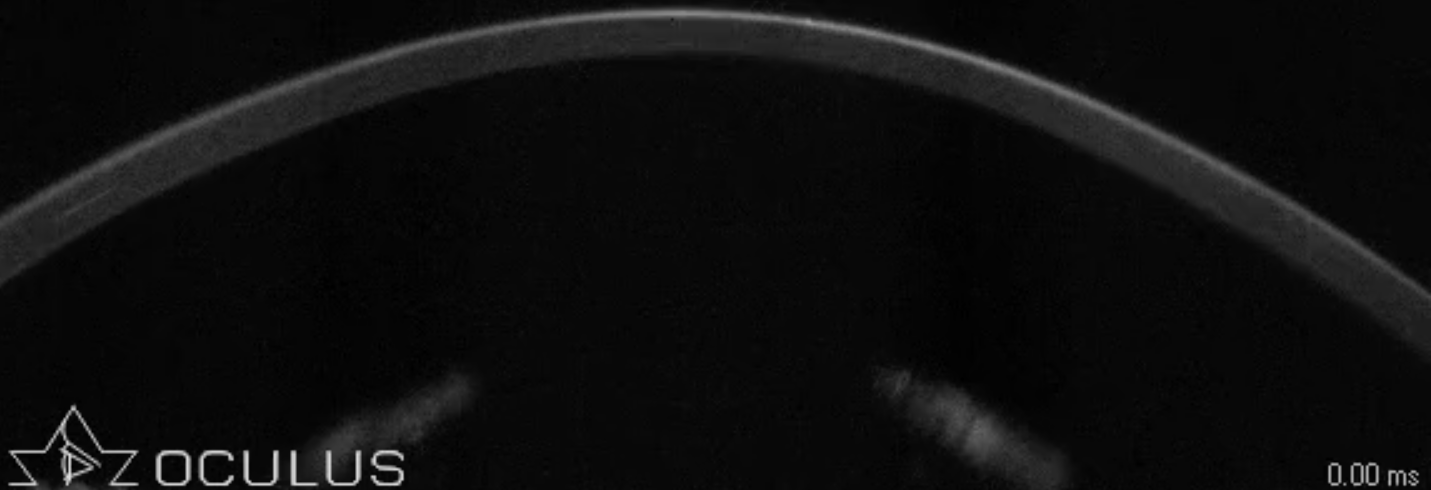
\includegraphics[width=1\linewidth]{figures/Compression/nodeform.png}
        \caption{Cornea Rest Image}
        \label{fig:nodeform}
    \end{figure}
    \begin{figure}[h]
        \centering
        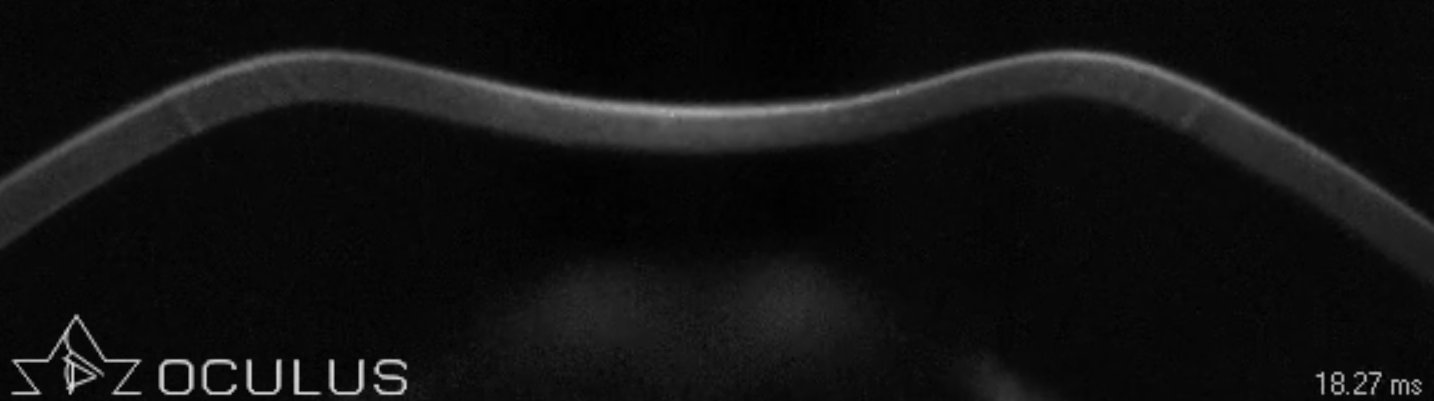
\includegraphics[width=1\linewidth]{figures/Compression/deform.png}
        \caption{Cornea After Some Elapsed Experiment Time}
        \label{fig:deform}
    \end{figure}
\end{itemize}
The idea we propose is that the
the fact that the cornea's shape on the problematic edge can be leveraged to determine ``how much cornea'' is added or removed with respect to frame 0 - the critical calibrating frame from which rest lengths are fetched. We can do this by setting a direction vector along which the surfaces on the edge ``slide'', so that when the edge moves down, it has slid along a vector of known direction, and the same when the points move back up during the expansion. This begs the following question.
\subsection*{How to choose the vector along which the edge segments slide?}
The cornea's motion contains translational under the global air puff's push, along with some contraction/expansion. To understand what the vector along which to slide the edge segments to determine to true motion of our extremities must look like, we consider the extreme cases below.
\begin{enumerate}
    \item The motion is entirely translational: this implies no horizontal displacement and consists of what we have already done (and want to evolve.) This is the case where the vector points perfectly upwards.
    \\\item The motion is entirely a perfect compression/expansion: a natural choice, in this case, is to slide the non-rotating segment at the edge along a normal to the surface. For instance, in this case, when the waveform fetcher notices a lowering of the left-most edge, it can calculate how much cornea on the edge is new and results from inward sliding and subsequently correctly relocate the extremity before minimizing with the frame's parameters which have a dynamic extremity adjustment.
\end{enumerate}
\textbf{We deduce that the true axis is an intermediate of the two. It could even be a spline based on a possibly false heuristic that the eye is pushed back before the muscle pushes it inwards. This is something to be tested empirically at first with eyes and a cursor because image thresholding prevents the automation of finding this movement hyperparameter, be it a spline or a vector. What will be automated is the movie-specific this axis or spline will take, which will be done in frame 0 calibration.}\\\\
This approach is yet to be down, and illustrations of which will be added to this document when it is done. We refrain from providing pseudo-code before the approach is more established in practice. We note, nonetheless, that this will be used only to move the extremity, as adding nodes and segments will not be compatible with the frame 0 calibration. \\\\
Note that this is easily extendable to the 3D case, much quicker than the energy algorithms, which are discussed in the Discussion section.
\section{Discussion}
To roughly summarize the above in a sentence, we've tried to leverage image processing and empirical heuristics to extract an evident characteristic energy proxy of corneas in hopes of finding something to distinguish between healthy corneas and those affected by disease. It goes without saying that we have yet to extend our methods to the surface or even volume cornea case once the fixes in the line element case are established.\\\\
Note that to extend the problem to higher dimension, we would have to change the notions of segment elements to surface elements and generalize the stretch and bending, which will require more computational power to handle these extra available movement directions. We look to start - once the 1D case is completed - to start with an axiosymmetric model, though this is not completely representative of the cornea, but could serve as a fine approximation (which is also very easy to do.)

\end{document}